\documentclass[12pt,a4paper]{article}
\usepackage[utf8]{inputenc}
\usepackage[T1]{fontenc}
\usepackage[francais]{babel}
\usepackage{amsmath}
\usepackage{amsfonts}
\usepackage{amssymb}
\usepackage{xcolor}
\usepackage{graphicx}
\usepackage[top=2.00cm]{geometry}
\usepackage{titlesec}
\usepackage{fancyhdr}
\usepackage{multicol}
\usepackage{titling}
\usepackage{mathtools}
\usepackage[hidelinks]{hyperref}
\graphicspath{{C:/Users/Sylvain/AppData/Roaming/texstudio/templates/user/}{./res/}}

%%modif des titres de section diminuer la taille
\renewcommand{\thesection}{\Roman{section}}
\titleformat{\section}
{\normalfont\bfseries\Large\scshape}{\thesection}{1em}{}
\titleformat{\subsection}
{\normalfont\bfseries\large}{\thesubsection}{1em}{}

\addto{\captionsfrench}{\renewcommand{\abstractname}{}}


%CONFIG
\author{Sylvain Finot}
\title{Initiation à la recherche :\\[5pt] \scshape "The Rattleback revisited"}
\date{\today}
\fancypagestyle{firststyle}{
	\fancyhf{}
	\setlength{\footskip}{2cm}
	\renewcommand{\headrulewidth}{0pt}
	\cfoot{\textcolor{lightgray}{\theauthor \ | Initiation à la recherche | Mars 2017}}
	\rfoot{\thepage}
}
\pagestyle{firststyle}

\makeatletter
\def\@maketitle{
	\begin{center}
		
		% NoLogo
		% \vspace*{+2cm}
		
		% Corner Logo
		% \begin{flushright}
		%  
\includegraphics[width=40mm]{logo_corner}\\[4ex]
		% \end{flushright}
		
		% Top Logo
		
\includegraphics[scale=0.3]{logo_top}
		
		
		{\LARGE \@title }\\[4ex]
		{\large \@author}\\[4ex]
		{\large \@date}\\[8ex]
		\rule{\linewidth}{0.4pt}
	\end{center}
}


%matrices configurables \begin{pmatrix}[2pt]
\renewcommand*\env@matrix[1][\arraystretch]{%
	\edef\arraystretch{#1}%
	\hskip -\arraycolsep
	\let\@ifnextchar\new@ifnextchar
	\array{*\c@MaxMatrixCols c}}
\makeatother


\begin{document}
	\maketitle
	\thispagestyle{firststyle}
	\begin{abstract}
		%todo mettre référence de American Journal of Physic
		Dans ce document, nous allons tenter d'expliquer au mieux l'étude du rattleback menée par William Case et Sahar Jalal.\\
		Leur article, \textit{"The rattleback revisited"}, paru dans The American Journal of Physics en 2014 traite du mouvement surprenant du rattleback. Bien que de nombreuses études aient été réalisées sur le rattleback, les auteurs mentionnent le fait que leur approche est beaucoup plus directe que celles déjà existantes au moment de la publication.\\
		
		Je vais donc essayer de traiter au mieux les points évoqués dans l'article et de synthétiser ce que j'ai compris avec mon niveau actuel de physique (3ème année de licence)
		%comprendre la démarche
		%voir les hypotheses
		%probleme LaTeX, beaucoup de temps si on veux etre precis
		%Rq: avec des bases de physique, on peut comprendre ce qui est fait sans forcement être capable de refaire tout les calculs.
	\end{abstract}
	\section{Introduction}
	Un rattleback, aussi appelé anagyre ou "Celtic stone", est un objet généralement en forme de canoë, qui a la particularité d'avoir un sens de rotation stable et un sens instable autour de l'axe vertical.
	\begin{figure*}[h]
		\centering
		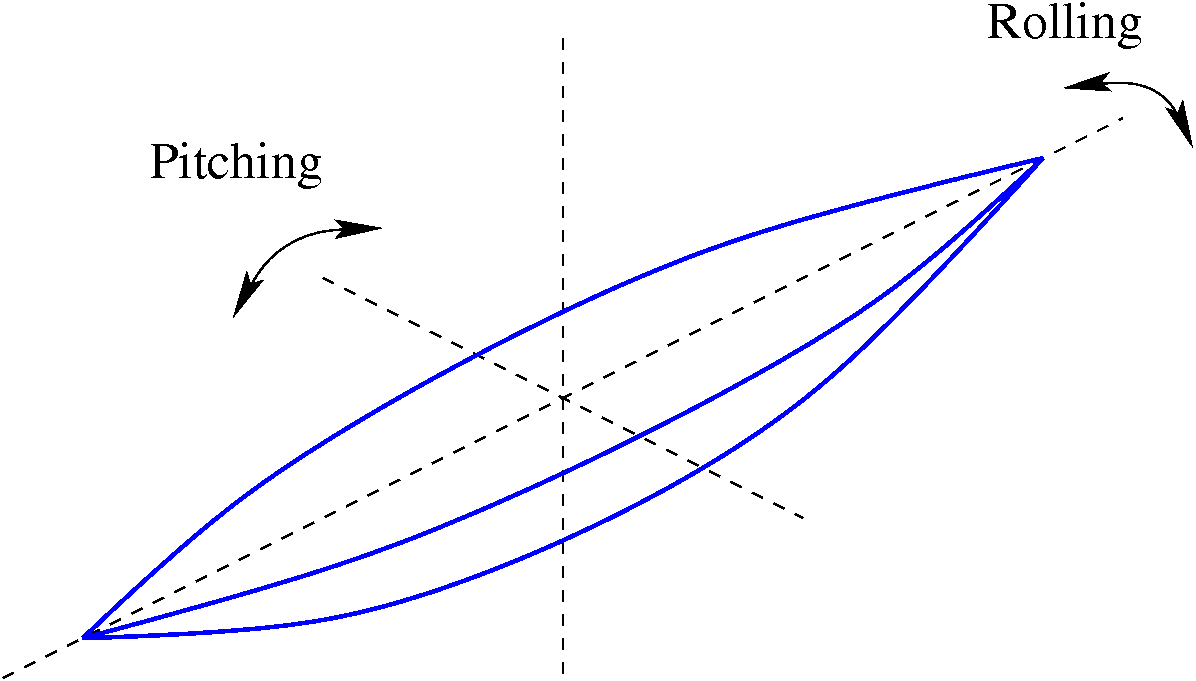
\includegraphics[scale=0.2]{Rolling-pitching}
		\caption[]{Représentation simpliste d'un rattleback}
		\label{fig:rolling-pitching}
	\end{figure*}
	
	Autrement dit, si on le met en rotation dans le "bon" sens, le mouvement continue jusqu'à immobilisation due aux forces de frottement. En revanche, si on le met en rotation dans le "mauvais" sens, très vite, l'objet oscille violemment ("rattle"), s'arrête, puis repart en sens inverse (i.e, le "bon" sens). Autre particularité, si on fait osciller le rattleback selon son petit axe (l'axe "pitching" \autoref{fig:rolling-pitching}), il entre en rotation dans le bon sens de rotation.
	
	Cet objet, par son mouvement paradoxal, est parfois retrouvé comme accessoire de magicien.
	Il a également fasciné grand nombre de physiciens et de mathématiciens. Les premières publications à ce sujet datent de 1896 par Gilbert Walker. La plupart des publications actuelles (XXI$^{e}$ siècle) se basent sur les travaux de Sir Hermann Bondi, "The Rigid Body Dynamics of Unidirectional Spin" de 1986.
	\subsection{Un problème de symétrie.}
	Bien que le mouvement du rattleback soit surprenant et fascinant, il n'y a rien de magique dans cet objet. Ses propriétés sont dues à un problème de symétrie. En effet, le rattleback est un objet asymétrique.
	
	Il existe deux manières de concevoir un rattleback : on peut décider de prendre une répartition de masse homogène, et dans ce cas, on brise la symétrie en modifiant le volume. On peut aussi choisir de conserver les symétries du volume et de "cacher" l'asymétrie en appliquant une répartition inhomogène de la masse avec par exemple des cavités. L'étude faite ici concerne le cas de répartition de masse homogène.
	
	\subsection{Démarche de l'étude}
	Afin de ne pas perdre le lecteur, je trouve important d'annoncer le plan de l'étude réalisée dans l'article.
	
	Le problème étant complexe, il est judicieux de découper l'analyse.
	La première partie consiste à étudier comment, à partir de rotation autour de l'axe vertical, le rattleback se met à osciller.
	Ensuite, les auteurs s'intéressent au cas contraire, c'est-à-dire, comment à partir d'oscillations le rattleback passe-t-il en rotation.
	
	C'est en réunissant les résultats des deux parties que l'on obtient une réponse relativement complète au problème.
	% il faut faire un certain nombre d'hypothèses pour pouvoir espérer le résoudre.
	% %todo : HYPOTHESES
	% On considère que le point de contact entre le rattleback et le support est au repos.
	% %Conservation de l'E (28 29)
	% 
	% Pour simplifier le traitement du problème, on peut le découper en deux parties.\\
	%  %D'une certaine manière, on peut voir cela comme une conversion d'énergie.\\
	% La deuxième partie, on s'intéresse au cas contraire, comment à partir d'oscillations le rattleback passe-t-il en rotation.
	\section{Oscillations}
	Dans cette première partie de l'étude, sans doute la plus complexe, on considère que le rattleback est initialement en rotation selon l'axe vertical sans aucune oscillation. On cherche alors à expliquer pourquoi et comment ce mouvement se transforme en oscillation.
	%L'idée est de mettre en équation le changement 
	En ce qui concerne l'aspect calculs, il faudra tenir compte du fait que le référentiel du centre de masse est en rotation par rapport au référentiel du laboratoire.\\
	Le repère utilisé a pour origine le centre de masse et comme axes, les axes de symétrie (en terme de distribution de masse).\\
	\begin{figure}[h]
		\centering
		\caption{Le rattleback vu de dessus. La répartition de masse ne respecte pas la symétrie de la forme.}{Crédit : Case \& Jalal}
		\label{fig:mass-repartition}
		\includegraphics[width=0.7\linewidth]{"mass repartition"}
	\end{figure}
	
	L'étude commence en s'intéressant au point de contact entre le rattleback et le support. On indique cette position par le vecteur $\vec{r}=(x,y,z)$. Après calculs, et en supposant que $x$ et $y$ ne sont pas trop éloignés de l'origine, on peut trouver une expression de la composante z.
	Cette équation semble être tirée des travaux d' Hermann Bondi. Il s'agit d'un développement obtenu à partir de l'équation d'un ellipsoïde. Les paramètres de cette équation sont décrits plus bas. 
	\begin{equation}
	z=a\left[ 1-\dfrac {1} {2}p\left( \dfrac {x} {a}\right) ^{2}-q\dfrac {xy} {a^{2}}-\dfrac {1} {2}s\left( \dfrac {y} {a}\right) ^{2}\right]
	\label{eq:z}
	\end{equation}
	
	On définit également le vecteur $\vec{u}$ qui est le vecteur unitaire normal à la surface, et qui est donc constant dans le référentiel du laboratoire. Concrètement, il s'agit "simplement" du vecteur unitaire définissant l'axe vertical dans le référentiel du laboratoire.\\
	
	En exprimant ce vecteur dans le référentiel du centre de masse, on obtient l'expression suivante :
	\begin{equation}
	\vec{u}=-\left(\dfrac{px+qy}{a},\dfrac{qx+sy}{a},1\right)
	\label{eq:uNormal}
	\end{equation}
	Où : \\
	\begin{tabular}{ll}
		$p$ &courbure selon $x$ (sans dimension)\\
		$s$ &courbure selon $y$ (sans dimension)\\
		$a$ &distance entre le centre de masse et le point le plus bas du rattleback au repos\\
		$q$ &facteur représentant l'asymétrie de l'objet (sans dimension)
	\end{tabular}
	\\
	
	L'expression est un peu compliquée, en effet le rattleback étant plus ou moins un demi-ellipsoïde, il n'est pas choquant de retrouver ces paramètres dans l'expression de $\vec{u}$. Une piste sur l'obtention de ce vecteur est détaillée \autoref{subsec:u}
	
	Par la suite, en utilisant la formule de Bour \eqref{eq:bour}, et disant que $\vec{u}$ est constant dans le référentiel du laboratoire \eqref{eq:uConstant}, on peut trouver une expression de $\vec{\omega}$\\(Calculs détaillés \autoref{subsec:omega})
	\pagebreak
	\begin{multicols}{2}
		\setlength\columnseprule{0.5pt}
		\noindent
		\begin{flalign}
		\dfrac{d\vec{A}}{dt}&=\dot{\vec{A}}+\vec{\omega}\times\vec{A}&
		\label{eq:bour}\\[1em]
		\dfrac{d\vec{u}}{dt}&=0&
		\label{eq:uConstant}
		\end{flalign}
		\vfill\null
		\columnbreak
		\noindent
		\begin{equation}
		\vec{\omega}=\dfrac{1}{a}\begin{pmatrix}[2]
		q\dot{x}+s\dot{y}-n(px+qy)\\
		-p\dot{x}+q\dot{y}-n(qx+sy)\\
		- na
		\end{pmatrix}
		\end{equation}
	\end{multicols}
	
	
	On peut alors trouver une expression de la vitesse, en effet : $\vec{v}=-\vec{r}\times\vec{\omega}$.\\
	\textbf{Remarques} :
	\begin{enumerate}
		\item Pour garder uniquement les termes du 1er ordre, cela revient à prendre $\vec{r}=(x,y,a)$ puisque $z=a$ au premier ordre.
		
		\item Si l'on veut être plus précis, la formule de Bour~\eqref{eq:bour} s'écrit de la manière suivante:  
		$$\left( \frac{d\vec{A}}{dt} \right)_{(R)}=\left ( \frac{d\vec{A}}{dt}  \right)_{(R')}+\vec{\Omega}_{(R'/R)}\wedge\vec{A}$$
		Ou R est le référentiel dit "fixe" (galiléen), R' le référentiel mobile et $\vec{\Omega}_{(R'/R)}$ le vecteur caractérisant la rotation entre R et R'.
	\end{enumerate}
	
	\vspace*{+1em}
	À partir de ce stade, la procédure devient plus "classique". On effectue un bilan des forces.\\
	En appliquant la deuxième loi de Newton:
	\begin{align*}
	\Sigma\vec{F}  &= m\vec{a}\\
	\iff\vec{F_c}+\vec{P} &= m\dfrac{d\vec{v}}{dt}
	\intertext{Où encore:}
	\iff\vec{F_c}-mg\vec{u}&=\dfrac{d\vec{p}}{dt}
	\end{align*}
	% l'accélération du barycentre dans le référentiel du laboratoire à l'aide de \eqref{eq:bour}.
	En prenant le produit vectoriel de l'expression ci-dessus avec $\vec{r}$ on obtient:
	\begin{equation}
	\dfrac{d\vec{L}}{dt}=m(\vec{r}\times\dfrac{d\vec{v}}{dt}+g\vec{r}\times\vec{u})
	\end{equation}
	Mais en utilisant la formule de Bour \eqref{eq:bour}, on peut également obtenir:
	$$\dfrac{d\vec{L}}{dt}=\dot{\vec{L}}+\vec{\omega}\times\vec{L}$$
	
	Ainsi, on obtient
	\begin{equation}
	m(\vec{r}\times\dfrac{d\vec{v}}{dt}+g\vec{r}\times\vec{u})=\dot{\vec{L}}+\vec{\omega}\times\vec{L}
	\end{equation}
	On a alors deux expressions de $d\vec{L}/dt$.\\
	En calculant les deux termes, on obtient deux équations différentielles (couplées) correspondant aux égalités des composantes $x$ et $y$ des deux termes.\\
	La composante z de $d\vec{L}/dt$ étant égale a 0 au premier ordre, on n'obtient pas d'équation.\\
	Les auteurs ont donc réussi à obtenir des équations du mouvement.\\
	
	Après un peu de mise en forme : 
	\begin{align}
	\label{eq:equa-diff-couplées1}
	(q\ddot{x}+s\ddot{y})\alpha-n(p\dot{x}+q\dot{y})(\alpha+\beta-\gamma)+n\dot{x}=\dfrac{g}{a}(-y(1-s)+qx)\\
	\label{eq:equa-diff-couplées2}
	-(p\ddot{x}+q\ddot{y})\alpha-n(q\dot{x}+s\dot{y})(\alpha+\beta-\gamma)+n\dot{y}=\dfrac{g}{a}(x(1-p)-qy)
	\end{align}
	Où les paramètres $\alpha,\beta,\gamma$ sont des paramètres sans dimension ayant pour expressions :
	\begin{equation*}
	\alpha=\dfrac{I_x}{ma^2}+1\qquad \beta=\dfrac{I_y}{ma^2}+1\qquad  \gamma=\dfrac{I_z}{ma^2}
	\end{equation*}
	Avec $I_x,I_y,I_z$ les moments d'inertie du solide.\\
	Ces équations étant assez fastidieuses à obtenir, on peut contrôler qu'elles sont cohérentes d'un point de vue dimensionnel (\autoref{subsec:dimension-equations}).\\
	
	Concernant la résolution, dans un premier temps les auteurs de l'article considèrent que le rattleback est au repos et qu'il ne possède pas d'asymétrie. (i.e $q=n=0$). Cela a pour effet de découpler les équations. On peut alors les résoudre plus simplement pour trouver : 
	
	(résolution \autoref{subsec:pulsations-propres}) \\
	\begin{align}
	\Omega_x^2&=\dfrac{g(1-s)}{as\alpha}\\[2ex]
	\Omega_y^2&=\dfrac{g(1-p)}{ap\alpha}
	\end{align}
	%todo ICI
	%ces expressions dépendent des moments d'inertie et de la courbure (s et p)
	%expressions calculés explicitement pour LEUR rattleback
	Par la suite, on reprend les équations différentielles en considérant l'asymétrie et la rotation. Le point le plus important pour les auteurs n'est pas la précision sur les pulsations, mais de mettre en évidence les termes qui déstabilisent les oscillations.
	
	Cette partie semble être relativement compliquée, après beaucoup calculs (non détaillés dans l'article),les auteurs arrivent à deux résultats :
	%todo expr 26 27
	%la rotation autour de z engenre des oscillations autours de x et y.
	%le sens instable depend de l'asymetrie q => en changeant le signe de q on inverse le sens instable (miroir)
	%$\Omega_x etant plus grand que \Omega_y, le rattleback entre d'avantage en rotation autour de x que autour de y
	\section{Énergie totale}
	Dans la partie précédente, on a vu que la rotation autour de l'axe z entraine des oscillations autour des axes y et z (pitching et rolling sur \autoref{fig:rolling-pitching}).\\
	Simplement en tenant compte du fait que l'énergie du système est conservée ou éventuellement dissipée par frottement pour tenir compte de la réalité, l'énergie d'oscillation provient donc de l'énergie de rotation.\\
	À terme, toute l'énergie de rotation est convertie en énergie d'oscillation. Le rattleback a donc cessé sa rotation autour de z et n'est plus qu'en oscillation.
	\begin{equation}
	E_{rot}+E_{x}+E_{y}=cst
	\end{equation}
	Avec les expressions obtenues par les auteurs, on peut montrer que l'énergie est essentiellement convertie en oscillation autour de $x$. Ce qui nous amène à la partie suivante de l'analyse.
	%oscillation alors rotation s'arrete.
	%Rattleback est majoritairement en oscillation autour de x
	\section{Rotation engendrée par des oscillations}
	%todo phrase bof
	Expliquer la rotation engendrée par des oscillations est plus simple que considérer l'inversement du sens de rotation.\\
	Pour expliquer ce phénomène, il faut considérer un mouvement d'oscillation autour de l'axe x, et aucune rotation autour de l'axe z.
	\begin{figure}
		\centering
		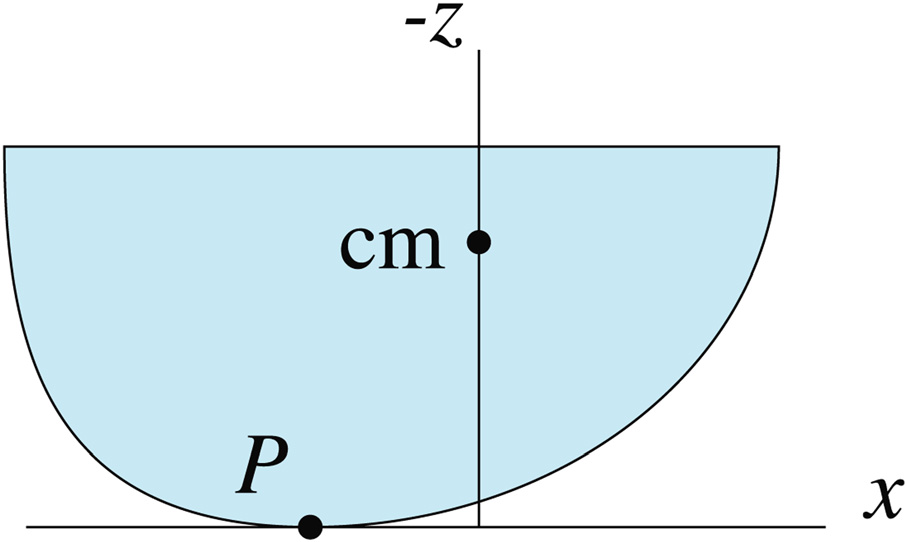
\includegraphics[width=0.7\linewidth]{res/coupe}
		\caption{Vu en coupe du rattleback pendant une oscillation autour de l'axe x}{Crédit : Case \& Jalal}
		\label{fig:coupe}
	\end{figure}
	Le centre de masse n'ayant pas la même abscisse selon les $x$, le poids de celui-ci crée un couple au point de contact. Voir figure~\ref{fig:coupe}. Ce couple tend à mettre en rotation le rattleback selon l'axe y.\\
	L'expression de ce couple au point P est donnée par :
	\begin{equation}
	\dfrac{dL_{py}}{dt}=-mgx=\dfrac{mgqy}{p}
	\end{equation}
	%todo détailler ca.
	Dans le référentiel du centre de masse, au centre de masse (i.e à l'origine) et au premier ordre, on a :
	\begin{align}
	%  \vec{v} &=\vec{r}\times\vec{\omega} \nonumber \\
	%    &\approx\left[0,0,a\right]\times\\
	v_x&=a \omega_y\\
	\intertext{D'où}
	\dfrac{dv_x}{dt}&=a\dfrac{d\omega_y}{dt}
	\end{align}
	L'accélération du centre de masse est équivalente à une force.
	Le couple produit par cette force tend à mettre en rotation le rattleback autour de l'axe z.\\
	
	\textbf{Remarque :} Un point pouvant prêter à confusion dans l'article est qu'il semblerait que les auteurs aient changé d'axe z en cours de route. En effet dans cette section, les résultats énoncés correspondent à des composantes z de vecteur en orientant celui-ci vers le haut.\\
	
	En considérant ce changement d'axe, on peut calculer la composante du couple tendant à mettre en rotation le rattleback autour de l'axe z.
	On obtient l'expression suivante :
	$$\tau=\dfrac{mgqy^2}{\beta p a}$$
	%Pour plus de détails dans les calculs, voir 
	%si CM accéléré <=> a une force qui s'exerce. La dite force est produite par le point de contacte.
	%On peut calculer le couple résultant de cette force : (32)
	
	
	
	%todo Résumé
	%trouver u (invariant) => trouver omega => trouver L => dL/dt = couple => equations du mouvement
	%ensuite on trouve une mise en oscillation
	%rotation => oscillation => rotation
	%résumer la démarche ?
	%Couper un probleme COMPLEXE en partie plus simples
	\section{Explications et vérifications des calculs}
	\label{sec:calculs}
	Dans cette section, on essaie de retrouver une partie des expressions données par les auteurs, en détaillant au possible les méthodes et les hypothèses pour y parvenir.\\
	Par alléger l'écriture, on pose la définition suivante :
	$$\dfrac{\partial}{\partial x}\equiv\partial_x$$ 
	\subsection{Vecteur normal}
	\label{subsec:u}
	La formule \eqref{eq:z} est liée à la forme d'ellipsoïde. Je n'ai pas compris pourquoi, mais on trouve le vecteur normal $\vec{u}$ \eqref{eq:uNormal} en prenant le gradient de \eqref{eq:z}. En effet :
	\begin{align*}
	\vec{\nabla}\cdot z &= \begin{pmatrix}
	\partial_x\\
	\partial_y\\
	\partial_z
	\end{pmatrix}
	\cdot
	a\left( 1-\dfrac {1} {2}p\left( \dfrac {x} {a}\right) ^{2}-q\dfrac {xy} {a^{2}}-\dfrac {1} {2}s\left( \dfrac {y} {a}\right) ^{2}\right)\\
	&=-\left(\dfrac{px+qy}{a},\dfrac{qx+sy}{a},1\right)
	\end{align*}
	\textbf{Remarque : } Il est dit dans l'article que $\vec{u}$ est le vecteur normal unitaire.
	\begin{quotation}
		<<upward-pointing unit normal u at that point is given, to first
		order in x and y, by...>>
	\end{quotation}
	Or, simplement en constatant que $u_z=1$, on en déduit que le vecteur n'est pas normé. Il faudrait prendre:
	\begin{align*}
	\vec{v} &=\dfrac{\vec{u}}{||u||}\\
	&=\dfrac{\vec{u}}{\sqrt{\left(\dfrac{px+qy}{a}\right)^2+\left( \dfrac{qx+sy}{a}\right)^2+1}}
	\end{align*}
	Cette petite "erreur" n'a pas d'importance sur la suite des calculs puisque la suite découle des équations suivantes :
	%todo : Faire ca sur 2 cols ?
	\begin{align*}
	\dfrac{d\vec{A}}{dt}&=\dot{\vec{A}}+\vec{\omega}\times\vec{A}\\[4pt]
	\dfrac{d\vec{v}}{dt}&=0
	\intertext{il vient alors :}
	\dfrac{d\vec{v}}{dt}&=\dot{\vec{v}}+\vec{\omega}\times\vec{v}\\
	&=\alpha\dot{\vec{u}}+\vec{\omega}\times\alpha\vec{u}\\
	&=\alpha(\dot{\vec{u}}+\vec{\omega}\times\vec{u})\\
	\intertext{D'où}
	\dot{\vec{u}}+\vec{\omega}\times\vec{u}=0 &\iff \dot{\vec{v}}+\vec{\omega}\times\vec{v}=0
	\end{align*}
	
	\subsection{Vecteur rotation $\vec{\omega}$}
	\label{subsec:omega}
	Pour trouver une expression de $\vec{\omega}$ nous avons besoin d'une propriété sur le produit vectoriel.
	\begin{equation}
	\vec{a}\times(\vec{b}\times\vec{c})=\vec{b}(\vec{a}\cdot\vec{c})-\vec{c}(\vec{a}\cdot\vec{b})
	\end{equation}
	Selon les équations \eqref{eq:bour} et \eqref{eq:uConstant} on a:
	\begin{align*}
	\dot{\vec{u}}+\vec{\omega}\times\vec{u}         &= 0\\
	\vec{u}\times(\dot{\vec{u}}+\vec{\omega}\times\vec{u})     &= 0\\
	\vec{u}\times\dot{\vec{u}}+\vec{u}\times(\vec{\omega}\times\vec{u})  &= 0\\
	\vec{u}\times(\vec{\omega}\times\vec{u})        &=-\vec{u}\times\dot{\vec{u}}\\
	\vec{\omega}(\vec{u}\cdot\vec{u})-\vec{u}(\vec{u}\cdot\vec{\omega})  &=\dot{\vec{u}}\times\vec{u}\\
	\intertext{En prenant $||\vec{u}||=1$ et en posant $\vec{u}\cdot\vec{\omega}\equiv n$}
	\vec{\omega}=\dot{\vec{u}}\times\vec{u}+n\vec{u}
	\end{align*}
	
	L'idée de poser $\vec{u}\cdot\vec{\omega}\equiv n$ m'a posé pas mal de problèmes de compréhension. Je me demandais quel en était l'intérêt, jusqu'à ce que je calcule explicitement $\vec{\omega}$.\\
	\bgroup
	\addtolength{\jot}{5pt}
	\begin{align*}
	\vec{\omega} &= \dot{\vec{u}}\times\vec{u}+n\vec{u}\\
	&=\begin{pmatrix}[2]\dfrac{p\dot{x}+q\dot{y}}{a}\\\dfrac{q\dot{x}+s\dot{y}}{a}\\0\end{pmatrix} \times \begin{pmatrix}[2]\dfrac{px+qy}{a}\\\dfrac{qx+sy}{a}\\1\end{pmatrix} -n\begin{pmatrix}[2]\dfrac{px+qy}{a}\\\dfrac{qx+sy}{a}\\1\end{pmatrix}\\
	%
	&=\begin{pmatrix}[2]
	\dfrac{q\dot{x}+s\dot{y}}{a}-n\dfrac{px+qy}{a}\\
	-\dfrac{p\dot{x}+q\dot{y}}{a}-n\dfrac{qx+sy}{a}\\
	\left(\dfrac{p\dot{x}+q\dot{y}}{a}\right)  \left(\dfrac{qx+sy}{a}\right)  - \left(\dfrac{q\dot{x}+s\dot{y}}{a}\right)  \left( \dfrac{px+qy}{a}\right)  - n
	\end{pmatrix}
	\end{align*}
	Il semblerait que les auteurs aient fait une hypothèse simplificatrice, les termes sous forme de fraction sont d'ordre 1. On a donc $\omega_z\approx-n$.\\
	D'où
	\begin{equation}
	\vec{\omega}=\dfrac{1}{a}\begin{pmatrix}[2]
	q\dot{x}+s\dot{y}-n(px+qy)\\
	-p\dot{x}-q\dot{y}-n(qx+sy)\\
	- na
	\end{pmatrix}
	\end{equation}
	\egroup
	Vérifions si on peut considérer les hypothèses comme valides :
	
	
	On rappelle que $x$ et $y$ représentent les coordonnées horizontales et verticales du point de contact par rapport au centre de masse. On se convint assez facilement que cet écart au centre de masse est petit par rapport aux dimensions de l'objet.On prendra en ordre de grandeur le millimètre.
	
	
	Nous n'avons pas d'information particulière sur les $\dot{x}$ et $\dot{y}$. Cependant les auteurs souhaitent résoudre le problème pour de petites vitesses.
	
	\begin{multicols}{2}
		\noindent
		\begin{align*}
		x&\approx y \approx 10^{-3}m&\\
		p&=0,923&\\
		s&=0,034&\\
		q&=0,1&\\
		a&=7,1.10^{-3}m&\\
		\end{align*}
		\columnbreak
		\begin{align*}
		\dfrac{qx+sy}{a}&\approx0,06\\[2em]
		\dfrac{px+qy}{a}&\approx0,27
		\end{align*}
	\end{multicols}
	\vspace*{-3em}
	On peut supposer que les termes en $\dot{x}$ et $\dot{y}$ sont également du même ordre.\\
	On peut considérer que $|\omega_z|\approx\pi$ (i.e 1/2 tour par seconde).\\
	L'hypothèse de considérer $\omega_z\approx-n$ semble alors plausible.
	
	%todo calc de v ?
	
	
	\subsection{Moment cinétique et moments de force}
	\label{subsec:moments}
	On cherche à obtenir une relation entre moments de forces (exprimés au barycentre) et moment cinétique. Les quantités sont exprimées dans le référentiel du laboratoire supposé galiléen.
	On part de:
	\begin{align*}
	\vec{L}     &= \vec{r}\times \vec{p}\\
	\iff\dfrac{d\vec{L}}{dt} &= \dfrac{d}{dt}(\vec{r}\times \vec{p})\\
	\iff\dfrac{d\vec{L}}{dt} &= \dot{\vec{r}}\times \vec{p}+\vec{r}\times \dfrac{d\vec{p}}{dt}\\
	\intertext{Or $\vec{p}$ et $\dot{\vec{r}}$ sont colinéaires $\implies \dot{\vec{r}}\times \vec{p} = 0$}
	\iff\dfrac{d\vec{L}}{dt} &= \vec{r}\times \dfrac{d\vec{p}}{dt}
	\end{align*}
	De plus $\dfrac{d\vec{p}}{dt}=\Sigma\vec{F}$ (2$^{\mathrm{eme}}$ loi de Newton)
	\begin{equation}
	\iff\dfrac{d\vec{L}}{dt} = \vec{r}\times\Sigma\vec{F}
	\end{equation}
	On retrouve en fait le théorème du moment cinétique.
	
	\subsection{Équations différentielles couplées}
	\label{subsec:dimension-equations}
	Vérifions que les équations \eqref{eq:equa-diff-couplées1} et \eqref{eq:equa-diff-couplées2} sont cohérentes d'un point de vue dimensionnel.\\
	On rappelle que les paramètres $p,s,q$ sont sans dimension.\\
	Il en est de même pour les paramètres $\alpha,\beta,\gamma$.\\
	En effet, ils s'écrivent sous la forme $\dfrac{I}{ma^2}$
	\begin{align*}
	\implies [\alpha]=[\beta]=[\gamma]=\dfrac{M.L^2}{M.L^2}=1
	\end{align*}
	On rappelle également que $n$ est par définition \eqref{subsec:omega} une vitesse angulaire $[n]=T^{-1}$.\\
	Ainsi chaque terme de \eqref{eq:equa-diff-couplées1} et \eqref{eq:equa-diff-couplées2} est homogène à une accélération.
	%\subsection{De l'oscillation à la rotation}
	
	\subsection{Pulsations propres}
	\label{subsec:pulsations-propres}
	Dans le cas où l'on considère l'objet au repos ($n=0$) et parfaitement symétrique ($q=0$), les équations \eqref{eq:equa-diff-couplées1} et \eqref{eq:equa-diff-couplées2} deviennent :
	
	\[
	\begin{cases}
	s\ddot{y}\alpha=\dfrac{g}{a}(-y(1-s))\\[2ex]
	-p\ddot{x}\alpha=\dfrac{g}{a}(x(1-p))
	\end{cases}
	\iff
	\begin{cases}
	\ddot{y}+\dfrac{g}{as\alpha}(1-s)y=0\\[2ex]
	\ddot{x}+\dfrac{g}{ap\alpha}(1-p)x=0
	\end{cases}
	\]
	On rappelle que par construction/définition : $0<p<1$ et $0<s<1$ et de même $g,a,\alpha$ sont strictement positifs.\\
	
	On peut donc poser
	\begin{align*}
	\Omega_x^2&=\dfrac{g(1-s)}{as\alpha}\\[2ex]
	\Omega_y^2&=\dfrac{g(1-p)}{ap\alpha}
	\end{align*}
	On reconnait alors les équations bien connues (oscillateurs harmoniques)
	\[
	\begin{cases}
	\ddot{y}+\Omega_y^2\ y=0\\[2ex]
	\ddot{x}+\Omega_x^2\ x=0
	\end{cases}
	\]
	Et donc $\Omega_x$ et $\Omega_y$ sont les pulsations propres de l'objet.
	\section{Conclusion}
	Pour conclure, ce travail d'analyse d'article scientifique m'a permis d'un certain nombre de choses.\\
	
	Tout d'abord, la façon dont est construite l'étude menée sur le rattleback me semble relativement naturelle. Je pense que cela vient du fait que nous nous familiarisons avec cette démarche scientifique dans nos études, quel que soit le domaine étudié. Ayant suivi qu'une brève introduction à la mécanique du solide, il m'a fallu admettre certains résultats, mais qui je trouve n'a pas été très gênant dans la compréhension de l'article. Cela m'a fait réaliser qu'avec les bases de physique acquis à la fin de la licence on peut comprendre ce qui est fait, suivre les étapes de calculs sans forcement être capable de les faire soi-même de A à Z.
	
	%comprendre la démarche
	%voir les hypotheses
	%probleme LaTeX, beaucoup de temps si on veux etre precis
	%Rq: avec des bases de physique, on peut comprendre ce qui est fait sans forcement être capable de refaire tout les calculs.
\end{document}
% Ils disent qu'ils n'ont pas forcément été plus loin dans l'analyse que leur prédeccesseur mais qu'a l'aide de bonnes approximations, ils ont pu grandement alleger les calculs et ainsi arrivé plus rapidement et facilement a un resultat.
%beaucoup d'autres articles qui traite le probleme en partant des memes bases mais par exemple préférence matricielle
%todo : ouverture sur autres objets étranges. Gömböc, disque d'euler, gyroscope